%% March 2018
%%%%%%%%%%%%%%%%%%%%%%%%%%%%%%%%%%%%%%%%%%%%%%%%%%%%%%%%%%%%%%%%%%%%%%%%%%%%
% AGUJournalTemplate.tex: this template file is for articles formatted with LaTeX
%
% This file includes commands and instructions

% There are two options for article format:
%
% PLEASE USE THE DRAFT OPTION TO SUBMIT YOUR PAPERS.
% The draft option produces double spaced output.
%

%% To submit your paper:
%\documentclass[draft,linenumbers]{agujournal2018}
\documentclass{agujournal2018}
\usepackage{apacite}
\usepackage{url} %this package should fix any errors with URLs in refs.

%%%%%%%
% \usepackage{trackchanges}
% uncomment the line above to use the TrackChanges package to mark revisions if needed.
% The trackchanges package adds five new LaTeX commands:
%
%  \note[editor]{The note}
%  \annote[editor]{Text to annotate}{The note}
%  \add[editor]{Text to add}
%  \remove[editor]{Text to remove}
%  \change[editor]{Text to remove}{Text to add}
%
% complete documentation is here: http://trackchanges.sourceforge.net/
%%%%%%%

%\draftfalse

% Now, type in the journal name: \journalname{<Journal Name>}
%

\journalname{Water Resources Research}

\begin{document}

%% ------------------------------------------------------------------------ %%
%  Title
\title{Network topology and rainfall controls on the variability of combined sewer overf\/lows and loads}

%% ------------------------------------------------------------------------ %%
%
%  AUTHORS AND AFFILIATIONS
%
%% ------------------------------------------------------------------------ %%

\authors{Gavan McGrath\affil{1,2,3,4},
Thomas Kaeseberg\affil{5}, 
Julian David Reyes Silva\affil{5},
James W. Jawitz\affil{6},
Frank Blumensaat\affil{7,8},
Dietrich Borchardt\affil{9},
Per-Erik Mellander\affil{1},
Kyungrock Paik\affil{10},
Peter Krebs\affil{5}, 
P. Suresh C. Rao\affil{11}
}

 \affiliation{1}{Environment, Soils and Land Use Department, Teagasc, Johnstown Castle, Wexford, Ireland}
 \affiliation{2}{Ishka Solutions, Nedlands, 6009, Australia}
 \affiliation{3}{School of Agriculture and Environment, The University of Western Australia, Perth, 6000, Australia}
  \affiliation{4}{Department of Biodiversity Conservation and Attractions, Kensington, 6151, Australia}
 \affiliation{5}{School of Civil and Environmental Engineering, Technische Universit\"at Dresden, Dresden, Germany}
 \affiliation{6}{Soil and Water Science Department, University of Florida, Gainesville, FL 32611, USA}
 \affiliation{7}{Eawag, Swiss Federal Institute of Aquatic Science and Technology, CH 8600 D\"ubendorf, Switzerland}
 \affiliation{8}{ETH Zurich, Institute of Environmental Engineering, 8093 Zurich, Switzerland}
 \affiliation{9}{Helmholtz Centre for Environmental Research UFZ, Magdeburg, Germany}
 \affiliation{10}{School of Civil, Environmental, and Architectural Engineering, Korea University, Seoul, South Korea}
 \affiliation{11}{Lyles School of Civil Engineering, Purdue University, West Lafayette, IN 47907, USA}

% Example: \correspondingauthor{First and Last Name}{email@address.edu}

\correspondingauthor{Gavan McGrath}{gavan.mcgrath@uwa.edu.au}

%% Keypoints, final entry on title page.
\begin{keypoints}
\item A parsimonious stochastic model is developed for CSO f\/lows and solute f\/luxes.
\item Uncalibrated stochastic model agrees with calibrated SWMM model.
\item Network structure and rainfall control CSO load variability.
\end{keypoints}

%% ------------------------------------------------------------------------ %%
%
%  ABSTRACT

%% \begin{abstract} starts the second page

\begin{abstract}
Water and pollutant f\/luxes from combined sewer overf\/lows (CSO) have a signif\/icant impact on receiving waters. The random nature of rainfall forcing dominates the variability of sewer discharges, pollutant loads, and concentrations. An analytical model developed here, shows how sewer network topology and rainfall properties variously impact the stochasticity of CSO functioning. Probability distributions of sewer discharge and concentration compare well with the results from a calibrated Storm Water Management Model in an application to a sewershed located in Dresden, Germany. The model is determined by only four parameters, three of which can be predicted a priori, two from the rainfall record and one from the network topology using geomorphological f\/low recession theory, while the fourth can be estimated from a short discharge time series.  The sensitivity of CSO and wastewater treatment loads to network structure suggests simple topologies may be more vulnerable to poor performance. The analytical model is useful for evaluating various CSO management strategies to reduce adverse impacts on receiving waters in a probabilistic setting.
\end{abstract}

%% ------------------------------------------------------------------------ %%
%
%  TEXT
%
%% ------------------------------------------------------------------------ %%

%%% Suggested section heads:
\section{Introduction}
With a preference for human settlement next to rivers globally \citep{Fang_2018}, wastewater discharges from urban areas have signif\/icant impacts on the health of riverine ecosystems and other human settlements downstream. A large number of cities globally have combined stormwater-sanitary sewer systems which discharge only mechanically treated sewage to aquatic and marine ecosystems during heavy rainfall. While urban wastewater treatment plants (UWWTPs) can take the majority of sewerage when present, combined-sewer overf\/low (CSO) discharges, rich in nitrogen, phosphorous, heavy metals, antibiotics, hormones and other sanitary pollutants, can have signif\/icant environmental impacts  \citep{David_2013,Phillips_2012}. Impacts on ecosystems arise from chemical (i.e. oxygen depletion, non-ionized ammonia peaks), and physical  (i.e. frequently increased bed shear) stresses which  depend to a large degree on local conditions \citep{borchardt1997urban}. Predicting the variability of CSO loads, concentrations and the frequency of events are key to understanding their impacts and for working towards resilient and sustainable urban drainage systems.

The variability of CSO functioning is a crucial component of its design. Key design criteria include: dilution rates in relation to dry weather f\/low; storage capacity in relation to design storms; an acceptable number of overf\/lows per year; a maximum tolerable pollution load; and a maximum CSO discharge, among others \citep{Riechel_2016}. Accounting for the stochastic nature of rainfall is one of the key challenges in CSO treatment design \citep{Geiger_1998}. On the other hand, the sewer network controls the travel time distribution and also inf\/luences the f\/lows and therefore the distribution of loads \citep{LHOMME_2004}. In the following, the hypothesis that both rainfall variability and the sewer network topology are signif\/icant controls on the statistical properties of CSO functions are elaborated.

\subsection{Rainfall Controls}
Rainfall variability is a dominant control of CSO event timing, event loads, and concentration variability \citep{COUTU2012477,Geiger_1998,Sandoval_2013}. Short intense rainfall can promote elevated loads in f\/irst f\/lush events \citep{Krebs_1999}. Long duration, low intensity events can lead to poorer ef\/f\/iciency at an UWWTP, reducing the relative contribution of CSOs to river pollution \citep{Phillips_2012}. Rainfall event intensities correlate with CSO water quantity and pollutant loads, while event duration and rain depth predict CSO pollutant concentrations \citep{Sandoval_2013}. Under the changing climatic conditions, the frequency of intense rainfall may increase, which brings concerns about an increasing frequency of CSO events \citep{Semadeni_Davies_2008,Sterk_2016}. These aspects of CSO performance are suited to treatment as a stochastic process, specif\/ically accounting for the statistical properties of the timing and magnitude of rainfall events on the hydrological response \citep{Botter_2009}.
     
\subsection{Network Topology and Discharge Variability}
Taking a nonlinear relationship between storage and runof\/f, $Q$, the continuity equation can be stated as \citep{Botter_2009}:
\begin{linenomath*}
\begin{equation}
\frac{dQ}{dt} = -k Q^\alpha+\xi(t)
\label{eq:one}
\end{equation}
\end{linenomath*}
where $k$ is related to the hydraulic residence time, $0< \alpha$ is a f\/low recession exponent. The rainfall, $\xi$, is assumed to follow a marked Poisson process with exponentially distributed times between events and event depths. From Eq. (\ref{eq:one}) the probability density function (pdf) for long-term temporal variability of $Q$ was previously derived and the shape of the pdf was shown to be strongly controlled by $\alpha$ \citep{Botter_2009}.

The topological properties of river networks have also been shown to be related to $\alpha$ \citep{Biswal_2014}. Through a decomposition of a river network into so-called independent links, a power-law relationship between the number of independent links $N(l)$ and the total lengths of those same links, $G(l)$, at a distance $l$ was derived: i.e. $N(l) \propto G(l)^\alpha$  \citep{Biswal_2010}. In rivers, at least, there appears to be an intrinsic relationship between the network structure, the hydrological response and the variability of discharge. 

Sewers share many topological characteristics with rivers \citep{Yang_2017}. Like rivers, sewers follow power laws in the area-distance relationship (Hack’s Law) and in the probability distribution of contributing area, with exponent values similar to those found in rivers \citep{Yang_2017}. A topological model also predicts runof\/f characteristics from sewers, as in rivers \citep{LHOMME_2004}. We therefore hypothesize that the topological properties of gravity-driven sewer networks will inf\/luence the pdf of discharges, as well as pollutant loads and concentrations.

%\begin{figure}[h]
% \centering
% 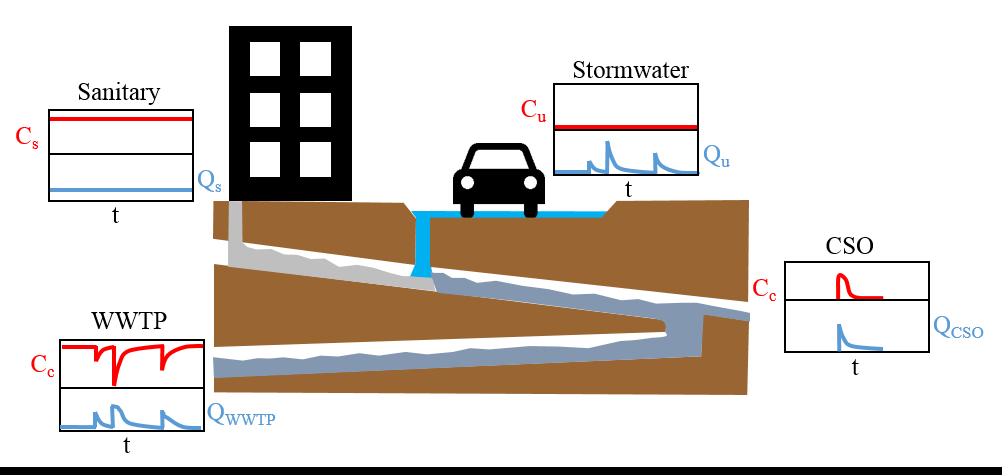
\includegraphics[width=30pc]{Fig1.pdf}
% \caption{Conceptual model of a combined sewer system. Sanitary flows, $Q_s$, of concentration $C_s$ are diluted stochastically by stormwater ($Q_u$, $C_u$) which then discharges intermittently to a CSO ($Q_{CSO}$, $C_c$) and continuously to a WWTP ($Q_{WWTP}$, $C_c$).}
% \label{figone}
% \end{figure}

\begin{figure}[h]
 \centering
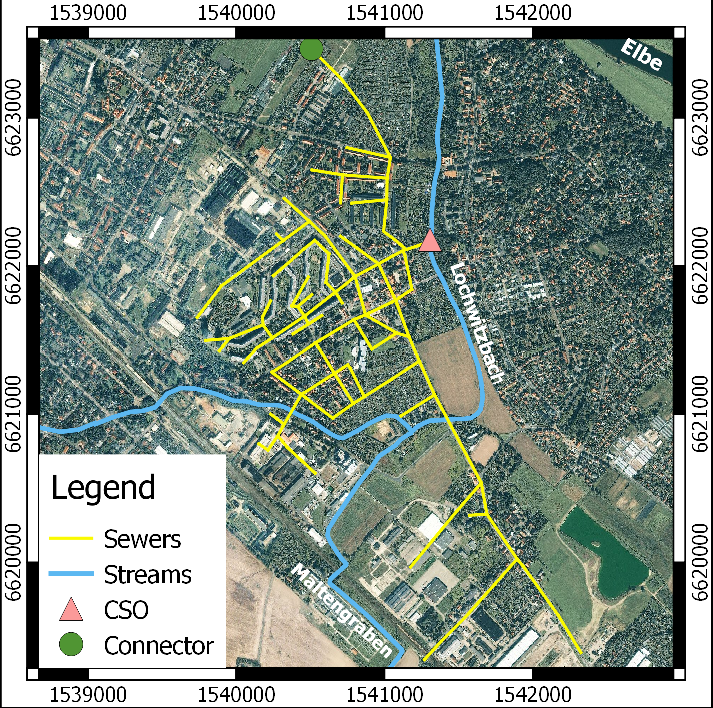
\includegraphics[width=15pc]{Fig2.pdf}
 \caption{The Lockwitzbach sewer network and CSO. Coordinates are UTM Zone 33 North.}
 \label{figtwo}
  \end{figure}

\subsection{A Utilitarian Perspective}
Clearly the structure of the sewer network and rainfall properties are important factors, together with regulations and/or guidelines, impacting upon CSO design and function. The manager of a sewer system might wonder what the use is to predict variability of a CSO system when she cannot change the rainfall properties or he can only tweak aspects of the structure of a sewer system at any one time. Firstly, in response, many parts of the world face the challenge of constructing sewer systems to keep pace with rapid urbanization \citep{xu2019urban}. As such there is a need for general design tools to plan future urban infrastructure as distinct from comprehensive hydrodynamic models solving the mass and energy balance equations for water and solute transport. Secondly managers of established systems more and more need to be aware of climate change impacts and to have a whole of catchment approach to managing sewer performance. This necessitates a systems-scale understanding of the transformation of rainfall variability into the variability of runoff production and sewer functioning.

Treating runof\/f as a stochastic process,  has led to recent insights into how urbanization is changing the statistical properties of runof\/f as well as the variability of urban wash-of\/f \citep{Daly_2014,Mej_a_2014}. A  stochastic approach was recently developed to evaluate the variability of water storage within, and discharges from a CSO tank \citep{Wang_2018}. The process descriptions of storage and discharge used by \citet{Wang_2018} are identical to those used to previously examine soil water storage \citep{McGrath_2007,Milly_1993} and the temporal clustering of threshold f\/low events \citep{Aquino_2017, Laio_2001, McGrath_2007}. Furthermore there have been recent advances in understanding how the network structure of rivers influences the hydrodynamics of discharge \citep{Biswal_2010}. As a result, we saw an opportunity to draw upon these new ideas in hydrology and apply them to improve the theoretical underpinnings of the practice of CSO management.  

In this contribution we develop analytical expressions for the pdfs of CSO discharges, loads and concentrations with parameters derived from rainfall and the structure of the sewer network. The pdfs compare favourably with the results of a calibrated Storm Water Management Model (SWMM). The model developed here allows a sewer system manager/designer to easily assess how changing rainfall patterns (e.g. climate change scenarios) or urban growth (e.g., expansion and redesign of the sewer network) would impact CSO functioning and the risks to urban rivers.
 
\section{Stochastic Analytical CSO Network Yield (saCSOny) Model}
\subsection{Discharges, Concentrations and Loads}
The combined f\/lows (and loads), $Q_c$ ($L_c$) at a CSO diversion are given by the sum of the sanitary f\/low (load), $Q_s$ ($L_s$), and urban stormwater f\/low (load), $Q_u$ ($L_u$):
\begin{linenomath*}
 \begin{eqnarray}
Q_c = Q_u + Q_s\\
\label{eq:two}
L_c =  C_c Q_c = L_u + L_s = C_u Q_u + C_s Q_s
\label{eq:three}
\end{eqnarray}
\end{linenomath*}
where $Q_u$ is the stochastic stormwater runoff and $Q_s$ is the sanitary discharge, $C_u$ is the solute concentration in stormwater, assumed to be constant and much smaller than the steady concentration in the sanitary flow, $C_s$.  Implicitly we will assume $L_u \ll L_s$ and that the above terms represent system averages and thus describe well-mixed conditions at the catchment-scale. Sanitary f\/lows typically display strong diurnal and weekly variability while stormwater f\/lows vary signif\/icantly at sub-hourly time scales during rainfall events. While $Q_s$ and $C_s$ are initially assumed constant this assumption is later relaxed, such that f\/luctuations in the sanitary f\/luxes can be taken into account. The dif\/ference between $Q_c$ and a threshold discharge, $Q_t$, at a CSO diversion, determines the CSO discharge, $Q_{CSO} = Q_c - Q_t$, and the load during a CSO event, $L_{CSO} = C_c Q_{CSO}$. The overflow structure is typically a weir and when the water level in the upstream pipe reaches a certain height, the weir overflows into the CSO pipes. These structures are constructed such that the flow directed towards the wastewater treatment plant depends on the upstream flow rate only to a minor extent. A simple threshold is therefore a good approximation to the hydrodynamics. The WWTP receives a f\/low, $Q_{WWTP} = Q_c - Q_{CSO}$, and a load, $L_{WWTP} = C_c Q_{WWTP}$. A stochastic model for $Q_u$ is described next from which pdfs for the f\/lows, loads and concentrations are derived. 

  
\subsection{Stormwater pdfs}
Starting with Eq. (\ref{eq:one}), \citet{Botter_2009} previously derived the pdf of discharges for rivers (the term $Q_u$ here). In relation to Eq. (\ref{eq:one}), when $\alpha = 1$, the storage - discharge relationship is described as a linear reservoir, such that f\/lows decrease exponentially with time during the recession phase. The pdf of $Q_u$ in this case is given by Eq. (\ref{eq:a1}). Flow recession in rivers, however, are often better described by power-laws \citep{Wittenberg_1999}. When $0 < \alpha < 1$ the nonlinearity is termed concave; when $1 < \alpha < 2$, a range often observed in rivers, the nonlinearity is termed convex and f\/inally, when $\alpha > 2$ the relation is termed hyperbolic. For concave recession the pdf is given by Eq. (\ref{eq:a2}) \citep{Botter_2009}. The pdfs of the convex and hyperbolic models have the same form as Eq. (\ref{eq:a2}) without the Dirac delta term. For the variables of interest ($Q_c$, $Q_{CSO}$, $Q_{WWTP}$, $C_c$, $L_{CSO}$, and $L_{WWTP}$) we can apply a change of variables to derive their pdfs from the pdfs for $Q_u$ (see Appendix A). 

\subsection{Accounting for Sanitary Discharge Variability}
To take into account the diurnal variation in sanitary flows ($Q_s$) and concentrations ($C_s$), they can be treated as random variables,independent of $Q_u$ and $C_u$. Using the marginal distribution rule, the pdf of $Q_c$ is related to the marginal distribution of $Q_c$, given $Q_s$ and the pdf of $Q_s$ i.e.:
\begin{linenomath*}
\begin{equation}
p_{q_c}\left(Q_c\right) = \int_{0}^{\infty} p_{q_c} \left(Q_c | Q_s\right) p_{q_s}\left(Q_s\right)\mathrm{d} Q_s
\label{eq:four}
\end{equation}
\end{linenomath*}
This is ef\/fectively a weighted average of the pdf of combined f\/lows (Eq. \ref{eq:a4}), where the weights are determined from the distribution of sanitary f\/lows ($p_{q_s}$). A short period of observed dry-weather f\/lows suf\/f\/ice to estimate $p_{q_s}$. The pdfs of discharges to the WWTP and from the CSO can be rescaled similarly. To derive the pdf of $C_c$ the same approach can be used together with the distribution of sanitary loads, $p_{L_s}$, or alternatively the joint distribution of $Q_s$ and $C_s$ using the marginal distribution of $C_c$ (Eq. \ref{eq:a10}), and the joint pdf of $Q_s$ and $C_s$ i.e.: 
\begin{linenomath*}
\begin{equation}
p_{c_c}\left(C_c\right) = \int_{0}^{\infty}\int_{0}^{\infty}p_{c_c}\left(C_c | Q_s ,C_s\right) p_{q_s c_s}\left(Q_s ,C_s\right) \mathrm{d}Q_s \mathrm{d}C_s
\label{eq:five}
\end{equation}
\end{linenomath*}
Practically this is achieved by sampling a short time series of dry-weather f\/lows $Q_{s}(t_i)$ and $C_{s}(t_i)$ at corresponding times then averaging the resulting ensemble of $p_{C_c}\left(C_c  | Q_s(t_i),C_s(t_i)\right)$ over the set of samples, at each concentration, $C_c$, then normalizing the result to obtain a pdf. The complete set of equations are presented in Appendix A. 

Next, the above model (defined by Eq \ref{eq:two}-\ref{eq:five} and \ref{eq:a1} - \ref{eq:a12}, which we refer to as saCSOny) is applied to a sewershed located in Dresden, Germany. The software R was used for data analysis \citep{RCore}. All code used in this paper is documented in Supplementary Material) and the SWMM input and output needed to run the scripts can be found at \url{https://doi.org/10.26182/5bbbff6fadf94}. The R code includes: scripts to numerically determine the pdfs and their corresponding cumulative distribution functions; analyse rainfall time series to determine the rainfall parameters; analyse SWMM input files to calculate $\alpha$ from the network properties; to analyse a discharge time series to conduct flow recession analysis; and to reproduce all figures in the main text and supplementary material.


   \begin{figure}[ht]
 \centering
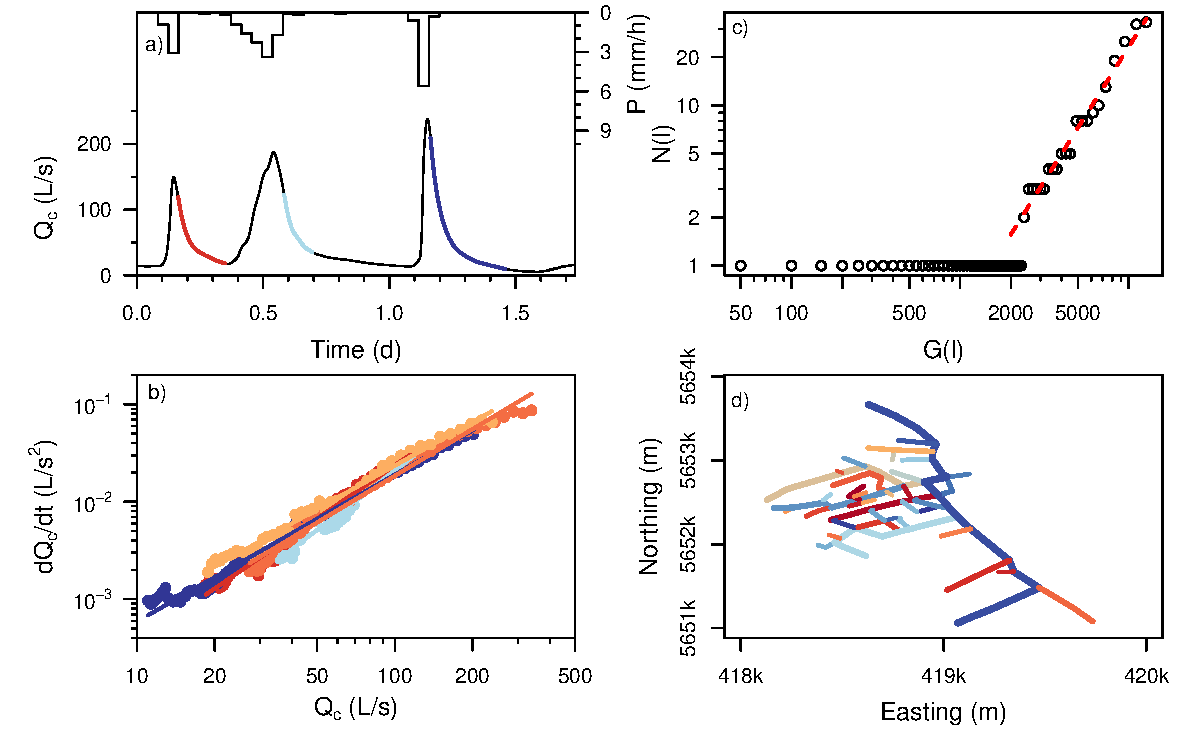
\includegraphics[width=30pc]{Fig4.pdf}
 \caption{Empirical f\/low recession analysis: a) discharge, $Q_c$, and rainfall, $P$, time series for three of the f\/ive events shown in (b); b) Linear regression of the logarithms of the rate of change in discharge, and mean discharge, i.e. $log(-dQ_c/dt) = log(k) +  \alpha log(Q_c)$ where the mean $\alpha = 1.7$ (Table S3); (c) The power law relation found between length and number of independent links i.e. $G(l) \propto N(l)^{1.7}$; and (d) The associated decomposed sewer network of independent links (color coded)  \citep{Biswal_2014}.}
 \label{figthree}
  \end{figure}
  
 \begin{figure}[ht]
 \centering
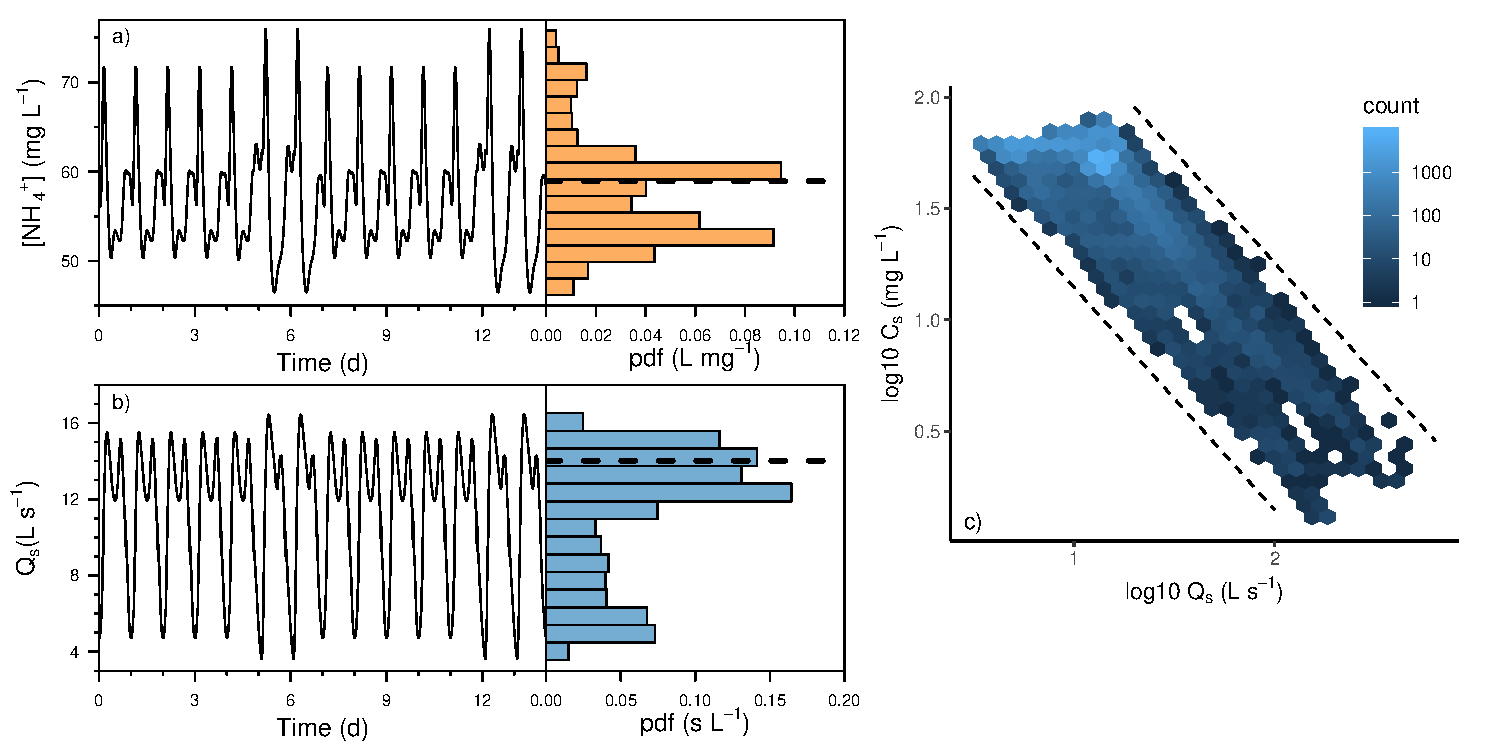
\includegraphics[width=30pc]{Fig3.pdf}
\caption{Characteristics of the sewer dynamics with: (a) Dry period discharges, $Q_s$ (and pdf $p_{q_s}$); (b) concentrations, $C_s$ $([NH_4^+])$ (and pdf $p_{c_s}$); and (c) the $C_c-Q_c$ relationship, bounded by $C_c \propto Q_c^{-1}$.}
 \label{figfour}
 \end{figure}


\section{Application}
\subsection{The Lockwitzbach Sewershed}
The Lockwitzbach sewer network, located in Dresden, Germany has a mean annual rainfall of 665 mm a\textsuperscript{-1} (1981-2010), a potential evaporation rate of 605 mm a\textsuperscript{-1} and a mean annual temperature of $9.4^\circ$C \citep{DWetter}. The sewershed has an area of 144.3 ha, with 36 ha of connected impervious surface. Wastewater from approximately 7,630 inhabitants and stormwater from primarily suburban land use is collected by 12.83 km of pipes. Extraneous water does not impact upon this sewer network \cite{Karpf_2011}. The CSO structure operates as a sidef\/low weir with a f\/low threshold of approximately 600 L s\textsuperscript{-1}. Excess water is discharged into the Lockwitbach, an urban stream that drains into the Elbe River. A gate prevents backf\/low from the stream or downstream pipes. The northern outlet of the sewershed provides a connection for transport to the central Dresden WWTP. 

\begin{table}[htb]
 \caption{saCSOny model parameters. $^{a}$JFM rainfall parameters are listed with other seasonal parameters listed in Table S2. Mean values for dry-spell sanitary parameters are tabulated. The 95\% conf\/idence interval is denoted by $\pm$.}
  \label{tab:one}
 \centering
 \begin{tabular}{l c l}
 \hline
  Parameter  & Value & Estimation method  \\
 \hline
   $\lambda$  & 0.30 d\textsuperscript{-1} & Rainfall event analysis$^{a}$\\
   $\gamma$  & 0.54 mm\textsuperscript{-1}  &\\
   $k$  & 2 $\pm$ 0.03 mm\textsuperscript{1-$\alpha$} d\textsuperscript{$\alpha-2$}  &  Flow recession.\\
   $\alpha$  & 1.7 $\pm$ 0.2 & Flow recession \& topology.  \\
  $Q_s$  & 11.3 L s\textsuperscript{-1}  & Empirical pdf of dry spell f\/lows.\\
   $C_s$  & 57.2 mg L\textsuperscript{-1} &   \\
   $C_u$ & 0 mg L \textsuperscript{-1} & Assumed.\\
 \hline
 \end{tabular}
 \end{table}

\begin{figure}[ht]
 \centering
 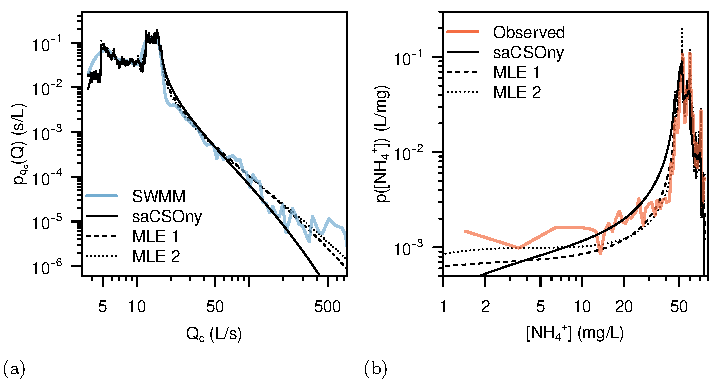
\includegraphics[width=30pc]{Fig5.pdf}
 \caption{Probability distributions of SWMM modeled and saCSOny predicted: (a) discharge, $Q_c$;  and (b) concentration, $C_c$. Parameters as in Table \ref{tab:one}. A posteriori f\/its of the pdf by maximum likelihood are also shown (MLE 1 where  $k$ was estimated with f\/ixed  $\alpha = 1.7$; and MLE 2 where both $k$ and  $\alpha$ were estimated, see Table S5).}
 \label{figfive}
 \end{figure}
 
A monitoring program of the joint Urban Observatory Dresden of Dresden University and the Helmholtz Centre for Environmental Research-UFZ under the Terrestrial Environmental Observation Initiative (TERENO) was established with the aims to analyze transport processes in sewer networks and the impacts of urban water management on river quality \citep{Helm2015, Wollschl_ger_2016}. For hydraulic and water quality simulations the open source software EPA-SWMM v. 5.1.011 was previously calibrated to this data \citep{Deb_2002,Kaeseberg_2018,Rossmann2010,steinberg2015}. The calibrated model was run with a time step of ten minutes, using rainfall at a similar temporal resolution. A 17 year simulation was produced providing modeled discharge and ammonia concentrations at the CSO junction with a 10 minute resolution. Further details can be found in Supplementary Material (Text S2, Figures S1 and S2).
 
\subsection{Parameter Estimation}
The climate parameters, $\lambda$ and $\gamma$, were determined from the precipitation time series (Supplementary Text S2, Table S2, Figures S3 - S5). These parameters describe the exponential probability distributions of the time between rainfall events and the magnitude rain events \citep{Rodriguez_Iturbe_1999}. A minimum rainfall-free period of 5 h, selected as the threshold to delineate distinct rain events, was chosen based upon the f\/low recession characteristics which typically had returned to near pre-event f\/low rates within this time-frame. Due to the seasonality of rainfall the analysis was separated into annual quarters def\/ined as January -– March (JFM), April -– June (AMJ), July -– September (JAS) and October -- December (OND). Precipitation totals for each event and the time between the start of events were determined and found to be approximately exponentially distributed for each quarter (Figures S3 and S4). The parameter $\lambda$ was estimated by multiplying the frequency of actual rainfall by the long term runof\/f coef\/f\/icient, 0.55. The parameters were estimated as the inverse of the mean of the time between rainfall events and the mean storm depth, respectively (Tables 2 and S2), equivalent to maximum-likelihood estimation. Potential for bias in the diurnal timing of events was assessed, with JFM and OND events distributed indistinctly from uniform distributions, indicating no bias in timing at a daily timescale (Figure S5). Events in AMJ and JAS were found to be signif\/icantly dif\/ferent from a uniform distribution by the Kolmogorov-Smirnov (KS) test, with a preference for early to mid-morning events as compared to the late evening. While present, this bias had little impact on the estimated pdfs.

The point in the network chosen to represent combined f\/lows was the junction immediately upstream of the pipe to the CSO structure (Figure \ref{figtwo}). The parameters, $k$ and $\alpha$, were estimated from the mean of f\/ive f\/low recession events \citep{Brutsaert_1977} (Figure \ref{figthree}, Table S3). Additional f\/low recession analyses were performed on 93 events (Table S4, Figure S6), selected with the criterion that the maximum discharge during the event was $>$160 L s\textsuperscript{-1} (i.e. approximately ten times the sanitary f\/low rate). Both analyses found a mean  $\alpha = 1.7$ and mean $k = 2$ mm\textsuperscript{1-$\alpha$} d\textsuperscript{$\alpha$-2} (Table \ref{tab:one}). A log-linear relationship (Figure S6c) between parameters was found between $k$ and $\alpha$. There was no evidence for a seasonal pattern in $k$ or a normalized $k$ \citep{Dralle_2015}. The geomorphological approach of \citet{Biswal_2014} was applied to estimate $\alpha$ using the topology of the sewer network (Figure \ref{figthree}c,d). This independently resulted in the same value, $\alpha = 1.7$, as the mean measured recession exponent (Text S5). Separately, maximum likelihood estimation (MLE) was applied to estimate $k$ (MLE 1) and both $k$ and $\alpha$ (MLE 2) using $p_{Q_c}$ (Table S5).
 
The sanitary discharge concentration has a characteristic diurnal and weekly periodicity (Figure \ref{figfour}a,b). A two-week long period of dry weather f\/lows was used to determine $Q_s$ and $C_s$, and from these their respective pdfs, $p_{Q_c}$ and $p_{C_c}$ (Text S6).  Across the entire time series the $C_c$ - $Q_c$ relationship is bound by strong dilution (i.e. $C_c \propto Q_c^{-1}$) with the variation of dry weather concentrations preserved over several orders of magnitude of $Q_c$ (Figure \ref{figfour}c), supporting the use of the well mixed assumption. Hysteresis is also evident, indicating that mixing is not perfect during individual events and thus apparently well mixed conditions emerge over the ensemble of flow events.

\subsection{Predicted pdfs of CSO Function}
The observed pdfs for JFM discharge and ammonia concentration [NH$_4^+$] agree well with the pdfs predicted from a priori estimated parameters (Figures \ref{figfive}; Figures S7 - S8, Text S7). A posteriori fits of the pdfs by MLE (Table S5) have very similar shapes. The multiple modes stem from the diurnal variation in sanitary f\/lows and the roughness of the pdfs stem from the application of Eq. \ref{eq:five} using a fine discretization of the empirical pdfs of $Q_s$ and $C_s$.  Importantly, the pdfs capture the long tails of both distributions which is necessary to correctly capture the load distribution for CSO events. 
 
Despite the similarity, one-sample KS tests reject the hypothesis that the empirical and model pdfs share the same distribution. As the KS tests develops statistics based upon the maximum deviation between the distributions, it is a conservative test. The failure of the test may stem from some clear dif\/ferences between the two distributions. For discharge in the range of f\/lows close to the upper end of sanitary f\/lows (20 L s\textsuperscript{-1}) the saCSOny model tends to slightly over predict the likelihood of discharges. Similarly for concentrations near the lower end of sanitary concentrations (30 mg L\textsuperscript{-1}). The latter may be due to the over-prediction of discharges. Small to medium rainfall events of long-duration and low intensity, not well described as Poisson shocks, may be another contributing factor. Hydrodynamic processes such as storage, pipe friction, and hydrodynamic dispersion may also have an inf\/luence. Despite some minor def\/iciencies the simple model is able to capture signif\/icant features of the pdfs, from a just two weeks of observed dry-weather f\/lows and a handful of f\/low recessions.
 
 \section{Sensitivity Analysis}
The ef\/fects of the four model parameters are illustrated in Figures \ref{figfive} - \ref{figseven} and Figures S9- S11, using those listed in Table \ref{tab:one} as base values and developing a sensitivity analysis by systematically varying the others.

\subsection{Network and Hydrodynamic Controls}
Flow recession has a signif\/icant impact upon CSO functioning (Figure \ref{figsix}). As $\alpha$ decreases the mode of $p_{Q_c}$ increases near $Q_s$, intermediate f\/lows become more probable and larger f\/lows less likely (Figure \ref{figsix}a). The pdf $p_{C_c}$ is a mirror image of $p_{Q_c}$, with lower concentrations less likely with higher $\alpha$. For small $\alpha$ there is the potential for the pdf to become bimodal (Figure \ref{figsix}b). Interestingly the probability of high $Q_{CSO}$ increases with decreasing $\alpha$ until $\alpha = 1$, and then with further decreases the probability of high discharges declines (Figure \ref{figsix}c). The frequency of CSO events f\/irst increases as $\alpha$ increases then for $\alpha > 1$ event frequency decreases again (Figure \ref{figsix}c). The distribution of WWTP discharges resembles that of $Q_c$, albeit truncated at the acceptance threshold, $Q_t$ (Figure \ref{figsix}d). For the parameters used, the pdfs of CSO load are relatively uniform for $\alpha > 1$ indicating a wide range of loads are equally probable (Figure \ref{figsix}e). The load probabilities decrease and increase in accord the the frequency of CSO discharge. The likelihood of smaller loads to the WWTP changes similarly with , peaking at $\alpha \sim 1.5$ in this instance (Figure \ref{figsix}f). 

Longer mean residence times (smaller $k$) increase the probability of: larger combined f\/lows; lower concentrations in combined f\/lows; higher f\/lows from CSOs; higher flows to WWTPs; and higher loads (Figure \ref{figseven}). Of the hydrological parameters $\alpha$ is a key inf\/luence on the probability a CSO is discharging (Figures \ref{figeight}). The parameter $k$,  controlling hydrodynamic response times, plays an inf\/luence the probability of CSO discharge at smaller values; that is, in catchments with longer mean residence times. The discharge threshold is also signif\/icant with declining likelihood of CSO discharge the higher the threshold and the higher the threshold the more signif\/icant are seasonal dif\/ferences in the rainfall (Figure S9). Some variability of the discharge threshold could be expected to occur due to the hydraulics of pipe flow. Some variability is also due to discharge measurement errors, as practical CSO construction often differs from principals of weir design for the purposes of flow measurement \citep{Ahm_2016}. The effect of a degree of variation in $Q_t$ on the frequency of CSO discharge can be inferred from Figure S9.  In the case of Lochwitzbach a 10 – 20\% variation in $Q_t$ would produce small differences in the order of magnitude estimate of the CSO frequency. Smaller thresholds however would result in larger absolute errors.



\begin{figure}[ht]
 \centering
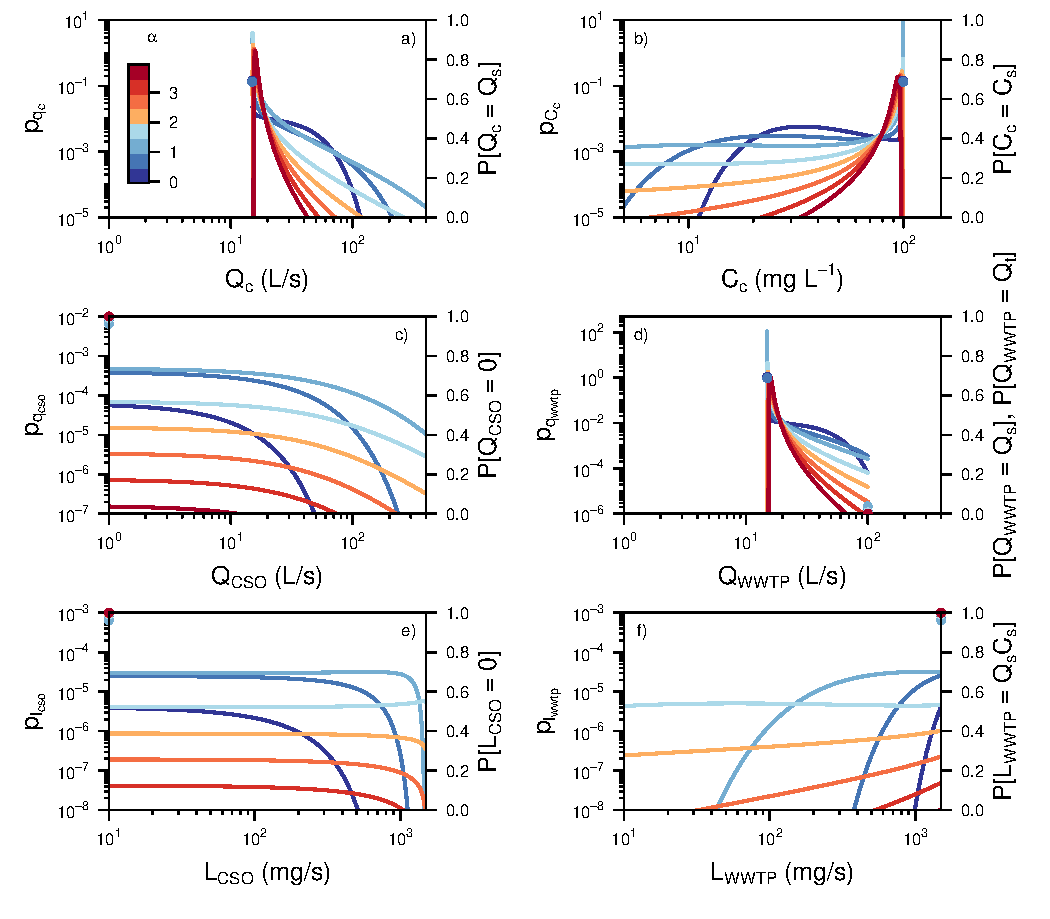
\includegraphics[width=30pc]{Fig6.pdf}
 \caption{The impact of the f\/low recession parameter, $\alpha$ , on pdfs of: (a) $Q_c$; (b) $C_c$; (c) $Q_{CSO}$; (d) $Q_{WWTP}$; (e) $L_{CSO}$; and (f) $L_{WWTP}$. Parameters used: $C_s$ = 100 mg L\textsuperscript{-1}, Qs = 15 L s\textsuperscript{-1}, Cu = 0 mg L\textsuperscript{-1}, k = 2 mm\textsuperscript{1-$\alpha$} d\textsuperscript{$\alpha$-2}, $\gamma$ = 0.45 mm\textsuperscript{-1}, $\lambda$ = 0.3 d\textsuperscript{-1}; $Q_t$ = 100 L s\textsuperscript{-1}. Lines denote the continuous part of the pdf (left axes) while the circles denote the atom of probability (right axes). For $L_{cso}$ and $Q_{cso}$ the points correspond to $L_{cso} = 0$ and $Q_{cso} = 0$.}
 \label{figsix}
 \end{figure}
 
 
\begin{figure}[ht]
 \centering
 \includegraphics[width=30pc]{Fig7.pdf}
\caption{Sensitivity analysis to the f\/low recession parameter, $k$, with $\alpha = 1.7$. All other parameters as in Figure \ref{figsix}.}
 \label{figseven}
 \end{figure}
 
 \subsection{Climate Controls}
Rainfall has a signif\/icant impact on function, as expected. Increasing rainfall frequency (also increasing total annual rainfall) shifts the pdfs of $C_c$ such that lower concentrations are more probable (Figure S10). This is in response to greater rainfall overall. The ef\/fect of increasing mean rain event depth ($1/\gamma$) is similar (Figure S11). Increasing rainfall frequency and mean rain event depth increases the probability of CSO events and higher loads as both contribute to greater overall rainfall (Figures \ref{figeight}b, S10, S11). The impact of fewer but more intense rainfall can be seen in the frequency of CSO events (Figure \ref{figeight}b). Climates of equal mean rainfall lie along lines with a slope of 1 in that f\/igure, and it can be seen that a shift from a high frequency, low intensity rainfall to a low frequency higher intensity rainfall results in an increasing probability a CSO is discharging.


\section{Discussion}
The saCSOny model quantif\/ied relative roles of climate and network parameters in controlling the statistics of CSO functions. The important role of climate is well known. Perhaps less well recognized is the signif\/icant ef\/fect that the network topology has upon the variability of CSO functioning.

\subsection{Network Controls}
For Lockwitzbach at least it was demonstrated that the topology of the sewers could predict $\alpha$. More work needs to be done to establish the extent to which this is more generally applicable to sewers. The empirical studies linking f\/low recession to topology have all been conducted on rivers to date \citep{Biswal_2014}. With sewersheds evolving from simple linear features at early stages of development, towards fractal objects with topological properties of rivers, we expect $\alpha$ to change as they grow \citep{Yang_2017}. \citet{Biswal_2014} suggested $\alpha \sim 1/(1-H)$, where $H \sim 0.6$ is Hack’s exponent. For sewers it has been shown $H$ decreases from $\sim 1$ to 0.6 as they matured \citep{Yang_2017}, which suggests $\alpha$ decreasing from $\infty$ to 2.5 during growth. While the relation suggested by \citet{Biswal_2010} may be valid for mature river networks, it may not be relevant for growing sewers. Intuition suggests that early on f\/low resembles a simple linear reservoir (i.e. $\alpha = 1$) and as the complexity of the network develops $\alpha$ likely increases. If this were the case the sensitivity analysis suggests that for the Lochwitzbach at least, high CSO loads and discharges tend to be more probable when $\alpha \sim 1$ (see Figure \ref{figfive}), thus poor performance of the CSO is more likely. 

For $k$ the expected changes seem to be clearer, as it is expected to decrease as the length of the pipe network and as the total area of connected impervious surface expands.  The parameter $k$ can be impacted by numerous factors. Longitudinal growth of the network would lengthen mean travel times of water and reduce $k$. Green infrastructure may also delay and lengthen travel times as a design goal. The results for Lockwitbach suggests that the frequency of CSO events would decline further were $k$ to decrease.  

A take-home message for a sewer manager is that alternative network structures will have varying flow recession exponents and, as a result, varying water quality outcomes. Designing the right structure, from a network perspective, has the potential to lower the costs and reduce the constraints to mitigate CSO impacts on receiving waters. The Lockwitzbach was the first sewer system in which $\alpha$ was predicted from the topology, so much more work needs to be done to evaluate this approach and identify its limitations in application to other sewersheds. Additionally, to design for growing infrastructure sewer manages would be further supported by providing them with knowledge as to how to design a network to achieve a  set of hydrodynamic parameters as well as to predict how these properties age as the sewersheds self-organise over time \citep{Semadeni_Davies_2008}.

\begin{figure}[ht]
 \centering
 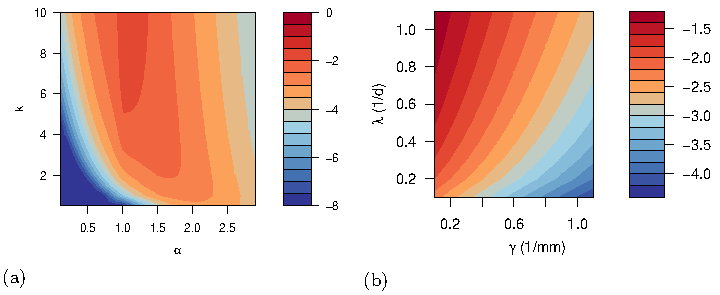
\includegraphics[width=30pc]{Fig8.pdf}
 \caption{Proportion of time (log10) a CSO discharges as a function of: (a) the topology/hydrodynamic parameters; and (b) the rainfall parameters. Parameters used include $Q_t = 100$ L s\textsuperscript{-1}, an impervious catchment area of 36 ha and for: (a) $\lambda = 0.3$ d\textsuperscript{-1}, $\gamma = 0.45$ mm\textsuperscript{-1}; and (b) $\alpha = 1.7$, $k = 2$  mm\textsuperscript{-0.7} d\textsuperscript{-0.3}.}
 \label{figeight}
 \end{figure}
 
\subsection{Climate Controls}
Regional, seasonal and inter-annual variations in rainfall properties vary signif\/icantly and may explain large dif\/ferences in CSO performance. We see (Figure \ref{figeight}) that increasing the likelihood of large rainfall events (smaller $\gamma$) leads to increased frequencies of CSO events \cite{Sterk_2016}. As the model assumes exponential distributions of rainfall depth and inter-even times it is best suited to describing what happens during typical conditions and may not be best at describing very rare events.

Catchment managers can't be expected to control the rainfall, as one reviewer pointed out, but it should be remembered that $\lambda$ is an effective rainfall event rate, incorporating the filtering of smaller, non-productive events, and thus the runoff coefficient.  Catchment managers can therefore directly influence the course of $\lambda$ by supporting green infrastructure, pervious paving, and managing the connectivity of impervious area, amongst others actions. For example, green infrastructure can increase inf\/iltration, increase detention storage, and reduce the peak f\/lows of urban runof\/f, thereby reducing CSO loads \citep{Riechel_2016}. Increased detention storage would decrease $\lambda$ though not signif\/icantly impact $\gamma$ \citep{Rodriguez_Iturbe_1999}. A $\lambda$ for green infrastructure, $\lambda_g$, can be estimated as: $\lambda_g = \lambda \exp⁡(-\gamma s)$, where $s$ is the ef\/fective catchment-scale detention storage added. In the case of Lockwitzbach the ef\/fect of adding an extra 1 mm of detention storage as green infrastructure would reduce the JFM $\lambda$ from 0.3 d\textsuperscript{-1} to 0.17 d\textsuperscript{-1}. Assuming that $\alpha$ and $k$ remain unchanged the frequency of CSO discharges would be expected to decrease approximately three-fold (Figures \ref{figeight}b, and S10). Natural multi-decadal variability as well as climate change related impacts on rainfall patterns have the potential to impact water quality outcomes \citep{mellander2018integrated, Semadeni_Davies_2008, Sterk_2016}. The saCSOny model offers the potential for sewer system managers to better plan for a mitigate these impacts.

\subsection{Mixing Assumptions}
The $C \propto Q^{-1}$ relationship, bounding the SWMM-simulated values (Figure \ref{figfour}), may be partly the result of the assumption in SWMM that individual pipes are completely mixed, high-dispersion reactors \citep{Rossmann2010}. This need not necessarily be the case at the scale of a sewershed, however in the case of the entire Lochwitzbach sewershed well-mixed conditions remain a reasonable approximation. Contrasting spatial distributions of stormwater and sanitary inf\/lows likely determine to what extent complete mixing is a reasonable approximation \citep{Krebs_1999}. Power law $C-Q$ relationships, $C = d Q^{-h}$ with $h < 1$, may be evidence of such incomplete mixing. Partial mixing could be introduced into Eq. \ref{eq:three} and distributions derived in a similar way (Text S1). Currently this would rely on an empirical $C-Q$ relationship to establish the mixing parameters which is somewhat unsatisfactory. As the f\/low recession exponent is estimated from the network topology it seems plausible that in the future related methods might be developed to predict $d$ and $h$ a priori, in a similar manner as has been done for f\/low recession \citep{Biswal_2014}.

\subsection{Assessing impacts on receiving waters}
The pdf of CSO loads can be used to estimate impacts upon receiving waters. Where guidelines specify CSO loads with respect to dry f\/low rates in a river \citep{Holzer_1998}, then the pdfs of CSO load can be integrated to estimate the probability of not meeting a dilution threshold. Alternatively, where the river responds on much longer time scales, say several days to rise and fall from a single rainfall event, then the pdf of a dynamic load threshold can be estimated assuming load and river discharge are independent random variables in a manner similar to Eq. (\ref{eq:four}). In the case of the small Lockwitzbach stream, the discharges would be strongly correlated with the sewer f\/lows at sub-daily time scales. In this case consideration of the covariance between stream and CSO discharges would be required.
The size of the sewershed in relation to the receiving water should also be a consideration in assessing the applicability of the saCSOny model. It is expected small to medium, gravity-driven sewersheds, with a small number of outlets would be most suitable, however additional research comparing saCSOny predictions with sewer performance would help clarify the situations where the model is and is not suitable.

\section{Conclusions}
A four-parameter analytical model has been developed here to explore hydrological and climate factors inf\/luencing the functioning of a simple combined sewer overf\/low system. We demonstrated that three of the parameters of the model can be estimated readily a priori from the climate and the structure of the sewer network and one parameter from a short time series of observed discharge by f\/low recession analysis. A signif\/icant f\/inding is that the f\/low recession exponent may be estimated from the sewer topology, and it signif\/icantly impacts variability of CSO function. This suggests that the statistical properties can be estimated from the design and a minimum of data without the need for solution of the full de Saint-Venant equations. Furthermore, relative contributions to variability from rainfall and the hydrodynamics/sewer structure can be disentangled. The equations derived here of\/fer new approaches to  rapidly assess options to mitigate CSO impacts on urban rivers. Future work is required to test the saCSOny model across diverse urban settings.

%Text here ===>>>

%% Enter Figures and Tables near as possible to where they are first mentioned:
%
% DO NOT USE \psfrag or \subfigure commands.
%
% Figure captions go below the figure.
% Table titles go above tables;  other caption information
%  should be placed in last line of the table, using
% \multicolumn2l{$^a$ This is a table note.}
%
%----------------
% EXAMPLE FIGURE
%
% \begin{figure}[h]
% \centering
% when using pdflatex, use pdf file:
% \includegraphics[width=20pc]{figsamp.pdf}
%
% when using dvips, use .eps file:
% \includegraphics[width=20pc]{figsamp.eps}
%
% \caption{Short caption}
% \label{figone}
%  \end{figure}

 


  

 
 
 
 
 
% ---------------
% EXAMPLE TABLE
%
 

%% SIDEWAYS FIGURE and TABLE
% AGU prefers the use of {sidewaystable} over {landscapetable} as it causes fewer problems.
%
% \begin{sidewaysfigure}
% \includegraphics[width=20pc]{figsamp}
% \caption{caption here}
% \label{newfig}
% \end{sidewaysfigure}
%
%  \begin{sidewaystable}
%  \caption{Caption here}
% \label{tab:signif_gap_clos}
%  \begin{tabular}{ccc}
% one&two&three\\
% four&five&six
%  \end{tabular}
%  \end{sidewaystable}

%% If using numbered lines, please surround equations with \begin{linenomath*}...\end{linenomath*}
%\begin{linenomath*}
%\begin{equation}
%y|{f} \sim g(m, \sigma),
%\end{equation}
%\end{linenomath*}

%%% End of body of article

%%%%%%%%%%%%%%%%%%%%%%%%%%%%%%%%
%% Optional Appendix goes here
%
% The \appendix command resets counters and redefines section heads
%
% After typing \appendix
%
%\section{Here Is Appendix Title}
% will show
% A: Here Is Appendix Title
%
\appendix
\section{The saCSOny Model}
The pdf for stormwater discharge in the case of linear case is \citep{Botter_2009}:
\begin{linenomath*}
\begin{equation} 
p_{q_u} \left(Q_u \right) = \frac{\gamma^{\frac{\lambda}{k}} Q_u^{\frac{\lambda}{k}-1}}{\Gamma\left(\frac{\lambda}{k}\right)}  \exp\left[-\gamma Q_u \right]
\label{eq:a1} 
\end{equation}
\end{linenomath*}
and for the nonlinear case \citep{Botter_2009}:
\begin{linenomath*}
\begin{equation}
p_{q_u}\left(Q_u \right) = \frac{K}{Q_u^{\alpha}} exp\left[-\frac{\gamma}{k}\frac{Q_u^{2-\alpha}}{2-\alpha} +\frac{\lambda}{k} \frac{Q_u^{1-\alpha}}{1-\alpha}   \right] + K \frac{k}{\lambda} \delta \left(Q_u\right)
\label{eq:a2}
\end{equation}
\end{linenomath*}
Using Eq. \ref{eq:a2} the remaining pdfs for f\/lows, loads and concentrations for the nonlinear case (the linear case is omitted for space as it can be derived similarly) can be derived using a change the variables, i.e.:
\begin{linenomath*}
\begin{equation}
p_y\left(Y\right) = p_x\left(f^{-1}\left(Y\right)\right) \left| \frac{\partial f^{-1}}{\partial Y} \right|	
\label{eq:a3}
\end{equation}
\end{linenomath*}
where $f^{-1}\left(Y\right)$ is the inverse of a function $Y=f\left(X\right)$ of a random variable, $X$, with probability density, $p_x \left(X\right)$, and $p_y\left(Y\right)$ is the pdf of $Y$. Applying a change of variables in the case of the combined f\/lows i.e. $Q_c = Q_s+Q_u$, gives the pdf of $Q_c$, as:
\begin{linenomath*}
\begin{equation}
p_{q_c}\left(Q_c \right) = K G\left(Q_c - Q_s \right) + K \frac{k}{\lambda} \delta \left(Q_u\right)
\label{eq:a4}
\end{equation}
\end{linenomath*}
where:
\begin{linenomath*}
\begin{equation}
G\left(x \right) = \frac{1}{x^{\alpha}} exp\left[-\frac{\gamma}{k}\frac{x^{2-\alpha}}{2-\alpha} +\frac{\lambda}{k} \frac{x^{1-\alpha}}{1-\alpha}   \right]
\label{eq:a5}
\end{equation}
\end{linenomath*}
The remaining pdfs are derived similarly. With a CSO event triggered when $Q_c > Q_t$ then the pdf of its discharge, $Q_{CSO}$, can be determined to be:
\begin{linenomath*}
\begin{equation}	
p_{q_{CSO}}\left(Q_{CSO} \right) = K G\left(Q_{CSO}+Q_t-Q_s \right) + P\left[Q_{C} < Q_t\right] \delta\left(Q_{CSO}\right)
\label{eq:a6}
\end{equation}
\end{linenomath*}
where:
\begin{linenomath*}
\begin{equation}	
P\left[ Q_{C} < Q_t\right] = \int_{0}^{Q_t} p_{q_c}\left(Q_c\right) \mathrm{d}Q_c 
\label{eq:a7}
\end{equation}
\end{linenomath*}
The pdf for $Q_{WWTP}$ is:
\begin{linenomath*}
\begin{eqnarray}\nonumber
p_{q_{WWTP}}\left(Q_{WWTP}\right) = K G\left( Q_{WWTP} - Q_s\right) + P\left[Q_t < Q_c\right]\delta\left(Q_{WWTP} - Q_t\right) + \\
P\left[Q_u = 0\right]\delta\left(Q_{u}\right)
\label{eq:a8}
\end{eqnarray}
\end{linenomath*}
where:
\begin{linenomath*}
\begin{eqnarray}
P\left[Q_t < Q_c\right] = \int_{Q_t}^{\infty} p_{q_c}\left(Q_c\right)\mathrm{d}Q_c 
\label{eq:a9}
\end{eqnarray}
\end{linenomath*}
and $P\left[Q_u=0\right]$ is given by the last term in Eq. (\ref{eq:a2}). The pdf of the concentration of ef\/f\/luent is:
\begin{linenomath*}
\begin{eqnarray}
p_{C_c | Q_s, C_s}\left(C_c \right) = K \frac{\left| C_u - C_s \right|}{\left(C_u - C_c \right)^2}  G\left(Q_s \left(\frac{C_s-C_c}{C_c-C_u }\right) \right) +  P\left[Q_u = 0\right] \delta\left(C_s - C_c\right) 
\label{eq:a10}
\end{eqnarray}
\end{linenomath*}
where we have written the pdf as a marginal distribution so as to recognize the possibility that $Q_s$ and $C_s$ may themselves display a degree of variability. While it is possible to derive the full pdf of CSO loads, for the sake of space and simplicity the case when the stormwater concentrations are negligible, i.e. $C_u\ll C_s$, is shown:
\begin{linenomath*}
\begin{eqnarray}\nonumber
p_{l_{CSO}} \left(L_{CSO} \right) = K  \frac{L_s}{\left(L_{CSO}-L_s \right)^2}    G\left(\frac{L_s}{\left(L_s - L_{CSO}\right)}  Q_t - Q_s \right)  + \\
P\left[Q_u \le Q_t \right]\delta\left(L_{CSO}\right)
\label{eq:a11}
\end{eqnarray}
\end{linenomath*}
where the sanitary load, $L_s = Q_s  C_s$ has been substituted. The pdf of WWTP loads is:
\begin{linenomath*}
\begin{eqnarray}
p_{l_{WWTP}} \left(L_{WWTP} \right) = K  \frac{Q_t L_s}{L_{WWTP}^2}    G\left(\frac{L_s}{L_{WWTP}}  Q_t - Q_s \right)  + \\
P\left[Q_u \le Q_t \right]\delta\left(L_s\right)
\label{eq:a12}
\end{eqnarray}
\end{linenomath*} 


%%%%%%%%%%%%%%%%%%%%%%%%%%%%%%%%%%%%%%%%%%%%%%%%%%%%%%%%%%%%%%%%
%
% Optional Glossary, Notation or Acronym section goes here:
%
%%%%%%%%%%%%%%
% Glossary is only allowed in Reviews of Geophysics
%  \begin{glossary}
%  \term{Term}
%   Term Definition here
%  \term{Term}
%   Term Definition here
%  \term{Term}
%   Term Definition here
%  \end{glossary}

%
%%%%%%%%%%%%%%
% Acronyms
   \begin{acronyms}
   \acro{CSO}
    Combined Sewer Overf\/low
   \acro{UWWTP}
    Urban Waste Water Treatment Plant
   \acro{SWMM}
    Stormwater Management Model
   \end{acronyms}

%
%%%%%%%%%%%%%%
% Notation
%   \begin{notation}
%   \notation{$a+b$} Notation Definition here
%   \notation{$e=mc^2$}
%   Equation in German-born physicist Albert Einstein's theory of special
%  relativity that showed that the increased relativistic mass ($m$) of a
%  body comes from the energy of motion of the body—that is, its kinetic
%  energy ($E$)—divided by the speed of light squared ($c^2$).
%   \end{notation}




%%%%%%%%%%%%%%%%%%%%%%%%%%%%%%%%%%%%%%%%%%%%%%%%%%%%%%%%%%%%%%%%
%
%  ACKNOWLEDGMENTS
%
% The acknowledgments must list:
%
% >>>>	A statement that indicates to the reader where the data
% 	supporting the conclusions can be obtained (for example, in the
% 	references, tables, supporting information, and other databases).
%
% 	All funding sources related to this work from all authors
%
% 	Any real or perceived financial conflicts of interests for any
%	author
%
% 	Other affiliations for any author that may be perceived as
% 	having a conflict of interest with respect to the results of this
% 	paper.
%
%
% It is also the appropriate place to thank colleagues and other contributors.
% AGU does not normally allow dedications.


\acknowledgments
PSCR, PK, GM and DB received f\/inancial support from the National Research Foundation of Korea (NRF) (grant 2015R1A2A2A05001592) to attend the Synthesis Workshop Dynamics of Structure and Functions of Complex Networks, held at Korea University in 2015. PSCR was partially funded by the Lee A. Reith Endowment in the Lyles School of Civil Engineering at Purdue University. GM and PEM received additional support from the Dif\/fuse Tools Project (grant 2016-W-MS-24) funded by the Environmental Protection Authority of Ireland. We thank Stadtentwaesserung Dresden for providing sewer network infrastructure and rainfall data. We further acknowledge the work of several research assistants at TU Dresden who contributed to the development of the SWMM model and the collection of reference data.

%% ------------------------------------------------------------------------ %%
%% References and Citations

%%%%%%%%%%%%%%%%%%%%%%%%%%%%%%%%%%%%%%%%%%%%%%%
% BibTeX is preferred:
%
% \bibliography{<name of your .bib file>}
%
% no need to specify bibliographystyle
%%%%%%%%%%%%%%%%%%%%%%%%%%%%%%%%%%%%%%%%%%%%%%%
\bibliography{agusample.bib}


% Please use ONLY \citet and \citep for reference citations.
% DO NOT use other cite commands (e.g., \cite, \citeyear, \nocite, \citealp, etc.).
%% Example \citet and \citep:
%  ...as shown by \citet{Boug10}, \citet{Buiz07}, \citet{Fra10},
%  \citet{Ghel00}, and \citet{Leit74}.

%  ...as shown by \citep{Boug10}, \citep{Buiz07}, \citep{Fra10},
%  \citep{Ghel00, Leit74}.

%  ...has been shown \citep [e.g.,][]{Boug10,Buiz07,Fra10}.


\end{document}



%More Information and Advice:

%% ------------------------------------------------------------------------ %%
%
%  SECTION HEADS
%
%% ------------------------------------------------------------------------ %%

% Capitalize the first letter of each word (except for
% prepositions, conjunctions, and articles that are
% three or fewer letters).

% AGU follows standard outline style; therefore, there cannot be a section 1 without
% a section 2, or a section 2.3.1 without a section 2.3.2.
% Please make sure your section numbers are balanced.
% ---------------
% Level 1 head
%
% Use the \section{} command to identify level 1 heads;
% type the appropriate head wording between the curly
% brackets, as shown below.
%
%An example:
%\section{Level 1 Head: Introduction}
%
% ---------------
% Level 2 head
%
% Use the \subsection{} command to identify level 2 heads.
%An example:
%\subsection{Level 2 Head}
%
% ---------------
% Level 3 head
%
% Use the \subsubsection{} command to identify level 3 heads
%An example:
%\subsubsection{Level 3 Head}
%
%---------------
% Level 4 head
%
% Use the \subsubsubsection{} command to identify level 3 heads
% An example:
%\subsubsubsection{Level 4 Head} An example.
%
%% ------------------------------------------------------------------------ %%
%
%  IN-TEXT LISTS
%
%% ------------------------------------------------------------------------ %%
%
% Do not use bulleted lists; enumerated lists are okay.
% \begin{enumerate}
% \item
% \item
% \item
% \end{enumerate}
%
%% ------------------------------------------------------------------------ %%
%
%  EQUATIONS
%
%% ------------------------------------------------------------------------ %%

% Single-line equations are centered.
% Equation arrays will appear left-aligned.




% To create multiline equations, use the
% \begin{eqnarray} and \end{eqnarray} environment
% as demonstrated below.
%If you don't want an equation number, use the star form:
%\begin{eqnarray*}...\end{eqnarray*}

% Break each line at a sign of operation
% (+, -, etc.) if possible, with the sign of operation
% on the new line.

% Indent second and subsequent lines to align with
% the first character following the equal sign on the
% first line.

% Use an \hspace{} command to insert horizontal space
% into your equation if necessary. Place an appropriate
% unit of measure between the curly braces, e.g.
% \hspace{1in}; you may have to experiment to achieve
% the correct amount of space.


%% ------------------------------------------------------------------------ %%
%
%  EQUATION NUMBERING: COUNTER
%
%% ------------------------------------------------------------------------ %%

% You may change equation numbering by resetting
% the equation counter or by explicitly numbering
% an equation.

% To explicitly number an equation, type \eqnum{}
% (with the desired number between the brackets)
% after the \begin{equation} or \begin{eqnarray}
% command.  The \eqnum{} command will af\/fect only
% the equation it appears with; LaTeX will number
% any equations appearing later in the manuscript
% according to the equation counter.
%

% If you have a multiline equation that needs only
% one equation number, use a \nonumber command in
% front of the double backslashes (\\) as shown in
% the multiline equation above.

% If you are using line numbers, remember to surround
% equations with \begin{linenomath*}...\end{linenomath*}

%  To add line numbers to lines in equations:
%  \begin{linenomath*}
%  \begin{equation}
%  \end{equation}
%  \end{linenomath*}



